\chapter{Building large SpiNNaker machines}
	
	\label{sec:building}
	
	Like any supercomputer, physically assembling a large SpiNNaker machine
	poses many practical challenges in terms of arranging, installing and
	maintaining the hundreds of metres of network cables required.  For
	conventional architectures and network topologies, techniques are well
	understood and embodied by industry standards such as TAI-942~\cite{tia2006}.
	SpiNNaker's use of the hexagonal torus topology renders existing approaches
	insufficient.
	
	In the first part of this chapter I extend existing techniques for mapping
	network topologies into standard data centre physical infrastructure to
	support the hexagonal torus topology. This mapping is designed to ensure that
	all cables are kept short (under \SI{1}{\meter}) to reduce costs and
	simplify the network hardware required. The techniques described introduce
	little overhead in cable length over existing torus wiring schemes
	and confirm the suitability of the hexagonal torus topology for real-world
	applications.
	
	The second part of this chapter uses SpiNNaker as a case study on the
	suitability of the mappings introduced in this chapter.  In this case study I
	consider various SpiNNaker systems ranging in size from desktop machines to
	multi-cabinet machine room installations. As well as validating the cabling
	schemes introduced in this chapter I also describe a new technique which
	improves the efficiency of the cable installation process.  As a consequence
	of SpiNNaker's fine-grained connectivity, the cabling is unusually dense,
	exacerbating the complexity of the cabling patterns to be installed. By
	exploiting network diagnostics hardware and on-board LEDs to guide cable
	installation, construction of large SpiNNaker machines takes a matter of
	hours rather than the days reported for other architectures. In addition,
	preliminary experiments suggest that neither the maintainability nor cooling
	performance of the system are hampered by the dense cabling employed.
	
	In this chapter, the term \emph{unit} refers to the smallest physical
	component between which network interconnection cables are installed. For
	example, in a SpiNNaker machine a unit is a 48-chip board while in a data
	centre network a unit might be a server blade.
	
	\section{Cabling non-hexagonal torus topologies}
		
		Na\"ive arrangements of torus topologies, hexagonal or otherwise, feature
		physically long `wrap-around' connections which connect units at the
		peripheries of the system. Long connections can be problematic for several
		reasons:
		
		\begin{description}
			
			\item[Performance:] Signal quality diminishes as cables get longer,
			requiring the use of slower signalling speeds, increased error
			correction overhead or more complex hardware.
			
			\item[Energy:] Some energy is lost in cables; longer cables lose more
			signal energy requiring higher drive strengths and/or buffering to
			maintain signal integrity.
			
			\item[Cost:] Shorter cables are cheaper than long ones.  Longer cables
			imply more cabling in a given space making the task of cable installation
			and system maintenance more difficult, increasing labour costs by as much
			as $5\times$~\cite{curtis12}.
			
		\end{description}
		
		In some cases, long connections in supercomputers may be eliminated by
		creative physical organisation of the system. For example, the distinctive
		`C'-shaped design of early Cray supercomputers was chosen to reduce the
		lengths of physical connections and thus improve system performance
		\cite{thocp13}. Unfortunately, this approach does not scale up in the
		general case and requires potentially expensive bespoke physical
		infrastructure.  Instead the need for long cables is often eliminated by
		folding and interleaving units of the network~\cite[chapter~5]{dally04}.
		This process is illustrated for a 1D torus topology (a ring network) in
		figure~\ref{fig:ring-folding}. A na\"ive arrangement of units in this
		topology results in a long cable connecting the units at the ends of the
		ring (figure~\ref{fig:ring-folding-row}).  To eliminate these long
		connections, half of the units are `folded' on top of the others
		(figure~\ref{fig:ring-folding-folded}) and then this arrangement of units
		is interleaved (figure~\ref{fig:ring-folding-interleaved}). This ordering
		of units requires no long cables while still observing the physical
		constraint that units must be laid out in a line.
		
		\begin{figure}
			\center
			\begin{subfigure}[b]{0.39\linewidth}
				\center
				\buildfig{figures/ring-folding-row.tex}
				\caption{A ring network}
				\label{fig:ring-folding-row}
			\end{subfigure}
			\begin{subfigure}[b]{0.24\linewidth}
				\center
				\buildfig{figures/ring-folding-folded.tex}
				\caption{Folded}
				\label{fig:ring-folding-folded}
			\end{subfigure}
			\begin{subfigure}[b]{0.35\linewidth}
				\center
				\buildfig{figures/ring-folding-interleaved.tex}
				\caption{Folded and interleaved}
				\label{fig:ring-folding-interleaved}
			\end{subfigure}
			
			\caption[Folding and interleaving a ring network.]%
			{Folding and interleaving a ring network to reduce maximum cable
			length.}
			\label{fig:ring-folding}
		\end{figure}
		
		The folding and interleaving process may be extended to $N$-dimensional
		torus topologies by folding each axis in turn. Since all axes are
		orthogonal in non-hexagonal topologies, the folding process only moves
		units along the axis being folded. Due to the non-orthogonality of the
		three axes of the hexagonal torus topology, this type of folding does not
		work. As figure~\ref{fig:failing-to-fold-hex-toruses} illustrates, folding
		along any axis results in connected units on opposing edges not being
		brought together. For example, when folding along the X axis, the two units
		marked with a green circle are moved closer together on the Y axis but
		remain apart on the X axis.
		
		\begin{figure}
			\center
			\begin{subfigure}[b]{0.24\linewidth}
				\center
				\buildfig{figures/failing-to-fold-hex-toruses-none.tex}
				\caption{Not folded}
				\label{fig:failing-to-fold-hex-toruses-none}
			\end{subfigure}
			\begin{subfigure}[b]{0.24\linewidth}
				\center
				\buildfig{figures/failing-to-fold-hex-toruses-x.tex}
				\caption{X}
				\label{fig:failing-to-fold-hex-toruses-x}
			\end{subfigure}
			\begin{subfigure}[b]{0.24\linewidth}
				\center
				\buildfig{figures/failing-to-fold-hex-toruses-y.tex}
				\caption{Y}
				\label{fig:failing-to-fold-hex-toruses-y}
			\end{subfigure}
			\begin{subfigure}[b]{0.24\linewidth}
				\center
				\buildfig{figures/failing-to-fold-hex-toruses-z.tex}
				\caption{Z}
				\label{fig:failing-to-fold-hex-toruses-z}
			\end{subfigure}
			
			\caption[Folding each axis of a hexagonal torus topology.]%
			{Schematics showing folding along each axis of a hexagonal torus topology
			failing to eliminate wrap-around connections.  Same-shaped-and-coloured
			dots show the endpoints of two example wrap-around connections.}
			\label{fig:failing-to-fold-hex-toruses}
		\end{figure}
	
	\section{Partitioning hexagonal torus topologies}
		
		The nodes in supercomputer networks are usually relatively small, for
		example a single chip. Tens of nodes are packed together into a single
		unit, such as a circuit board or server blade, to simplify assembly and
		share common power and cooling resources~\cite{gilge14,ajima12}. In
		commercial supercomputers built on non-hexagonal torus topologies, each
		unit's nodes represent a hypercube partition of the overall topology as
		illustrated in figure~\ref{fig:hypercube-partitioning}
		\cite{chen11,ajima12}.
		
		An analogous `parallelogram' partitioning scheme exists for hexagonal torus
		topologies, however, this results in imbalanced connectivity requirements
		between neighbouring partitions. In
		figure~\ref{fig:parallelogram-partitioning}, for example, the partitions
		above, below, left and right of the central partition are connected by
		seven node-to-node connections each while the partitions above-right and
		below-left are connected by just a single connection each. To simplify
		assembly, connections between all nodes in a pair of neighbouring
		partitions are often made by a single cable. If connectivity requirements
		are imbalanced, as in this example, this may mean multiple connector types
		may be required, increasing design complexity.
		
		To avoid connectivity imbalance, SpiNNaker uses a `wrapped triple'
		partitioning scheme~\cite{davidsonWiring}, as illustrated in
		figure~\ref{fig:wrapped-triple-partitioning} and explained in detail in
		appendix \ref{sec:partitioning}. In this partitioning scheme, the same
		number of connections connect all six neighbouring units. As explained in
		the appendix, a hexagonal torus topology is constructed from groups of
		three partitions.
		
		\begin{figure}
			\center
			\begin{subfigure}[b]{0.32\textwidth}
				\center
				\buildfig{figures/hypercube-partitioning.tex}
				\caption{2D hypercube}
				\label{fig:hypercube-partitioning}
			\end{subfigure}
			\begin{subfigure}[b]{0.32\textwidth}
				\center
				\buildfig{figures/parallelogram-partitioning.tex}
				\caption{Parallelogram}
				\label{fig:parallelogram-partitioning}
			\end{subfigure}
			\begin{subfigure}[b]{0.32\textwidth}
				\center
				\buildfig{figures/wrapped-triple-partitioning.tex}
				\caption{Wrapped triple}
				\label{fig:wrapped-triple-partitioning}
			\end{subfigure}
			
			\caption[Partitioning of torus topologies into units.]%
			{Partitioning of non-hexagonal (a) and hexagonal (b and c) torus
			topologies into units.}
			\label{fig:partitioning-options}
		\end{figure}
		
		For completeness, both parallelogram and wrapped triple partitioning are
		considered in this chapter even though SpiNNaker uses wrapped triple
		partitioning. The parallelogram partitioning scheme may be more appropriate
		for architectures where connections between nodes in neighbouring
		partitions do not share a single connector. In addition, in architectures
		where a unit corresponds to a single node, this can be treated as a $1
		\times 1$ parallelogram partition.  This special case occurs in
		coarse-grained architectures and Networks on Chip (NoCs) where nodes are
		not grouped together into multi-node units.
	
	\section{Folding \& interleaving hexagonal toruses}
		
		To exploit the folding technique used by non-hexagonal topologies, the
		units in a hexagonal torus topology must be mapped into a space with
		orthogonal coordinates. The choice of transformation to an orthogonal
		coordinate system can have an impact on how physically far apart logically
		neighbouring units are in the final arrangement. A good mapping should
		attempt to reduce `distortion' which moves adjacent units apart in the
		final folded and interleaved arrangement.
		
		In this section I propose two transformations which map hexagonal
		arrangements of units into a 2D orthogonal coordinate space. The first
		transformation, `shearing', is general purpose but introduces some
		distortion. The second transformation, `slicing', is less general but can
		introduce less distortion than shearing and therefore may lead to shorter
		cable lengths.
		
		Both the slicing and shearing transformations are carried out in two steps:
		
		\begin{description}
			
			\item[Rectangularisation] Units are transformed from being laid out in a
			parallelogram into a rectangular arrangement. The specific transformation
			used is the key difference between the slicing and shearing
			transformations.
			
			\item[Uncrinkling] Units are mapped into a 2D coordinate system without
			gaps between units.
			
		\end{description}
		
		\subsection{Rectangularisation}
			
			The hexagonal torus topology is illustrated in
			figures~\ref{fig:hex-to-plane-node-native} and
			\ref{fig:hex-to-plane-native} for parallelogram-partitioned units and
			wrapped triple units respectively. The first step in the folding process
			is to rearrange units so that they form a rectangle using one of two
			techniques: shearing or slicing.
			
			\begin{figure}
				\center
				\begin{subfigure}[b]{0.32\linewidth}
					\center
					\buildfig{figures/hex-to-plane-node-native.tex}
					
					\caption{Original}
					\label{fig:hex-to-plane-node-native}
				\end{subfigure}
				\begin{subfigure}[b]{0.32\linewidth}
					\center
					\buildfig{figures/hex-to-plane-node-shear.tex}
					
					\caption{Sheared}
					\label{fig:hex-to-plane-node-shear}
				\end{subfigure}
				\begin{subfigure}[b]{0.32\linewidth}
					\center
					\buildfig{figures/hex-to-plane-node-slice.tex}
					
					\caption{Sliced}
					\label{fig:hex-to-plane-node-slice}
				\end{subfigure}
				
				\caption[Rectangularisation of parallelogram partitioned toruses.]%
				{Rectangularisation of parallelogram partitioned hexagonal
				toruses. Thin lines show wrap-around links. Pointy-topped hexagons
				represent parallelogram partitioned units.}
				\label{fig:hex-to-plane-node}
				
				% XXX: Force these figures together.
				
				%\end{figure}
				%
				%\begin{figure}
				
				\center
				\begin{subfigure}[b]{0.32\linewidth}
					\center
					\buildfig{figures/hex-to-plane-native.tex}
					
					\caption{Original}
					\label{fig:hex-to-plane-native}
				\end{subfigure}
				\begin{subfigure}[b]{0.32\linewidth}
					\center
					\buildfig{figures/hex-to-plane-shear.tex}
					
					\caption{Sheared}
					\label{fig:hex-to-plane-shear}
				\end{subfigure}
				\begin{subfigure}[b]{0.32\linewidth}
					\center
					\buildfig{figures/hex-to-plane-slice.tex}
					
					\caption{Sliced}
					\label{fig:hex-to-plane-slice}
				\end{subfigure}
				
				\caption[Rectangularisation of wrapped triple partitioned toruses.]%
				{Rectangularisation of wrapped triple partitioned hexagonal
				toruses. Thin lines show wrap-around links.  Flat-topped hexagons
				represent wrapped triple partitioned units.}
				\label{fig:hex-to-plane}
				
				% And force these together!
				
				%\end{figure}
				%
				%\begin{figure}
				
				\center
				\begin{subfigure}[b]{0.3\linewidth}
					\center
					\buildfig{figures/slicing-examples-5x5.tex}
					\caption{$5\times5$}
				\end{subfigure}
				\begin{subfigure}[b]{0.3\linewidth}
					\center
					\buildfig{figures/slicing-examples-5x7.tex}
					\caption{$5\times7$}
				\end{subfigure}
				\begin{subfigure}[b]{0.3\linewidth}
					\center
					\buildfig{figures/slicing-examples-5x10.tex}
					\caption{$5\times10$}
				\end{subfigure}
				
				\caption[Patterns of wrap-around connections in sliced systems.]%
				{Schematics showing the patterns of wrap-around connections in sliced
				systems of various aspect ratios.}
				\label{fig:slicing-examples}
			\end{figure}
			
			The shearing technique applies a \SI{30}{\degree} shear transformation to
			distort the arrangement of units so that the X and Y axes of the
			hexagonal torus topology become orthogonal. This transformation leads to
			a rectangular arrangement of units as illustrated in figures
			\ref{fig:hex-to-plane-node-shear} and \ref{fig:hex-to-plane-shear}.
			
			The shear transformation introduces some distortion causing connections
			between units in the Z axis to become $\sqrt{2} \times$ longer. The
			transformation does not alter the pattern of wrap-around connections:
			long connections between units on the extreme left and right sides and
			the top and bottom remain, along with a single connection between the
			bottom left and top right units.
			
			The slice transformation aims to avoid the elongation of the Z axis by
			moving the units without distorting their layout. Units protruding from
			the left-hand-side of the parallelogram are `sliced off' and moved into
			the matching gap on the opposite side as illustrated in figures
			\ref{fig:hex-to-plane-node-slice} and \ref{fig:hex-to-plane-slice}. This
			transformation does not introduce any distortion but changes the pattern
			of wrap-around connections. Connections from left to right remain while
			the connections between the top and bottom units now criss-cross
			(figure~\ref{fig:slicing-examples}).  The proportion of connections going
			from bottom-left to top-right and from bottom-right to top-left varies
			depending on the aspect ratio of the topology. Only certain patterns of
			wrap-around links can be eliminated by folding and, as we shall see
			later, this limits us in which network topologies can be rectangularised
			by slicing.
			
		\subsection{Uncrinkling}
			
			Before folding can occur, the rectangularised arrangements of units
			produced in the previous step must be mapped into a 2D grid. Applied to
			parallelogram partitions, the shear transformation results in a mapping
			into a 2D grid with no further distortion
			(figure~\ref{fig:uncrinkling-node-sheared}). For other combinations of
			transformation and partitioning scheme, the units do not exactly fit a 2D
			grid. Instead, the units form `crinkled' rows or columns which may be
			`uncrinkled' (straightened out) to fit a regular 2D grid as illustrated in
			figures~\ref{fig:uncrinkling-node-sliced}~--~\ref{fig:uncrinkling-sliced}.
			
			\begin{figure}
				\center
				\begin{subfigure}[b]{0.48\linewidth}
					\center
					\buildfig{figures/uncrinkling-node-sheared.tex}
					
					\caption{Parallelogram units, sheared}
					\label{fig:uncrinkling-node-sheared}
				\end{subfigure}
				\begin{subfigure}[b]{0.48\linewidth}
					\center
					\buildfig{figures/uncrinkling-node-sliced.tex}
					
					\caption{Parallelogram units, sliced}
					\label{fig:uncrinkling-node-sliced}
				\end{subfigure}
				
				\vspace{1cm}
				
				\begin{subfigure}[b]{0.48\linewidth}
					\center
					\buildfig{figures/uncrinkling-sheared.tex}
					
					\caption{Wrapped triple units, sheared}
					\label{fig:uncrinkling-sheared}
				\end{subfigure}
				\begin{subfigure}[b]{0.48\linewidth}
					\center
					\buildfig{figures/uncrinkling-sliced.tex}
					
					\caption{Wrapped triple units, sliced}
					\label{fig:uncrinkling-sliced}
				\end{subfigure}
				
				\vspace{1em}
				
				\caption[Uncrinkling units into a 2D grid.]%
				{Uncrinkling rectangularised arrangements of units into a 2D
				grid. Thick lines show how crinkled rows and columns of units are
				uncrinkled.  Annotations show how the relative positions of units
				change after uncrinkling.}
				\label{fig:uncrinkling}
			\end{figure}
			
			%% XXX: Does this make things clearer or not?
			%In the figure, the labels show the positions of individual units before
			%and after uncrinkling. We will use these later in \S\ref{sec:distortion}
			%to calculate the overhead introduced by uncrinkling.
		
		\subsection{Folding}
			
			Once a regular 2D grid of units has been formed, this may be folded in
			the conventional way as illustrated in figure~\ref{fig:folding-sheared}.
			Folding once along each axis eliminates long connections crossing from
			left to right, top to bottom and from the bottom-left corner to the
			top-right corner. Any shear-transformed network may be folded this way
			since its wrap-around connections always follow this pattern.
			Slice-transformed networks may only be folded like this when their aspect
			ratio is $1:2$ when the pattern of wrap-around links is the same as a
			shear-transformed network.
			
			\begin{figure}
				\begin{subfigure}{\linewidth}
					\center
					\buildfig{figures/folding-sheared.tex}
					\caption{Sheared systems and $1:2$ sliced systems}
					\label{fig:folding-sheared}
				\end{subfigure}
				
				\vspace{1em}
				
				\begin{subfigure}{\linewidth}
					\center
					\buildfig{figures/folding-sliced.tex}
					\caption{$1:1$ sliced systems}
					\label{fig:folding-sliced}
				\end{subfigure}
				
				\caption[Elimination of long wrap-around links by folding.]%
				{Schematic illustrating elimination of long wrap-around links
				during folding. In each example a single link has been highlighted to
				aid in following the process.}
				\label{fig:folding}
			\end{figure}
			
			When `square' networks (i.e. those with a $1:1$ aspect ratio) are sliced,
			the network must be folded \emph{twice} along the Y axis as in
			figure~\ref{fig:folding-sliced} to eliminate the criss-crossing
			wrap-around links. It is not possible to eliminate wrap-around links from
			sliced networks with other aspect ratios by folding.
			
			After folding, the units are interleaved, yielding a 2D arrangement of
			units in which no connection spans the width or height of the system. The
			maximum connection distance is constant for any network allowing the
			topology to scale up.
		
		\subsection{Choosing a transformation}
			
			\label{sec:distortion}
			
			In each step of the transformation from hexagonal torus to a folded and
			interleaved 2D grid, the distances between connected units may increase.
			When designing a system, the transformation with the least distortion
			should be used to minimise the average length of the cables required.
			
			By referring to figure~\ref{fig:uncrinkling} again, it is possible to
			calculate the overhead introduced by each type of transformation.  For
			example, to compute the overhead introduced by the slicing transformation
			when applied to units composed of wrapped triples we consider
			figure~\ref{fig:uncrinkling-sliced}. The uncrinkling pattern used to
			transform this topology is a repeating pattern of two units, a pair of
			which have been labelled $1$ and $2$ respectively. Unit $1$ is
			immediately surrounded by the six units labelled $a$, $b$, $c$, $2$, $g$
			and $h$. Unit $2$ is surrounded by the units $1$, $c$, $d$, $e$, $f$ and
			$g$.  Before the transformation, the distance between units is $1$; after
			the transformation is applied this is not always the case. Folding and
			interleaving into $f_x$ columns and $f_y$ rows also introduces overhead.
			For each pair of previously neighbouring units in the example, their
			distances after folding may be computed as follows:
			
			\begin{equation*}
				\begin{aligned}[c]
					D_{1\,\leftrightarrow{}\,a} &= \sqrt{f_x^2 + f_y^2} \\
					D_{1\,\leftrightarrow{}\,b} &= f_y \\
					D_{1\,\leftrightarrow{}\,c} &= \sqrt{f_x^2 + f_y^2} \\
					D_{1\,\leftrightarrow{}\,2} &= f_x \\
					D_{1\,\leftrightarrow{}\,g} &= f_y \\
					D_{1\,\leftrightarrow{}\,h} &= f_x
				\end{aligned}
				\hspace{2cm}
				\begin{aligned}[c]
					D_{2\,\leftrightarrow{}\,1} &= f_x \\
					D_{2\,\leftrightarrow{}\,c} &= f_y \\
					D_{2\,\leftrightarrow{}\,d} &= f_x \\
					D_{2\,\leftrightarrow{}\,e} &= \sqrt{f_x^2 + f_y^2} \\
					D_{2\,\leftrightarrow{}\,f} &= f_y \\
					D_{2\,\leftrightarrow{}\,g} &= \sqrt{f_x^2 + f_y^2}
				\end{aligned}
			\end{equation*}
			
			From these values, mean and maximum connection distances may be
			calculated. The expressions for each combination of partitioning scheme
			and transformation are as follows:
			
			\begin{align*}
				D_{\textrm{mean}}=&
					\begin{cases}
						\frac{7f_x + 3\sqrt{f_x^2 + f_y^2} + \sqrt{(2f_x)^2 + f_y^2}}{9} &
							\textrm{if sheared wrapped triple units}\\
						\frac{f_x + f_y + \sqrt{f_x^2 + f_y^2}}{3} &
							\textrm{otherwise}\\
					\end{cases} \\
				D_{\textrm{max}}=&
					\begin{cases}
						\sqrt{(2f_x)^2 + f_y^2} &
							\textrm{if sheared wrapped triple units}\\
						\sqrt{f_x^2 + f_y^2} &
							\textrm{otherwise}
					\end{cases}
			\end{align*}
			
			\begin{table}
				\center
				\begin{tabular}{lcc}
					\toprule
					                                 & $1:2$  & Other \\
					\addlinespace
					\multirow{2}{*}{Parallelogram}   & \textbf{Either} & \textbf{Shear}\\
					                                 & \footnotesize $D_\textrm{mean}\approx2.28 \quad D_\textrm{max}\approx2.83$
					                                 & \footnotesize $D_\textrm{mean}\approx2.28 \quad D_\textrm{max}\approx2.83$\\
					\addlinespace
					\multirow{2}{*}{Wrapped triples} & \textbf{Slice}  & \textbf{Shear}\\
					                                 & \footnotesize $D_\textrm{mean}\approx2.28 \quad D_\textrm{max}\approx2.83$
					                                 & \footnotesize $D_\textrm{mean}\approx3.00 \quad D_\textrm{max}\approx4.47$\\
					\bottomrule
				\end{tabular}
				
				\caption{Recommended transformations for folding hexagonal toruses.}
				\label{tab:transform-recommended}
			\end{table}
			
			Using these formulae it is possible to determine which approach --
			shearing or slicing -- results in the lowest mean and maximum cable
			lengths and thus which technique should be used. This is summarised in
			table~\ref{tab:transform-recommended}.
	
	\section{A SpiNNaker case study}
		
		As the only known large-scale hexagonal torus-based architecture, SpiNNaker
		is a good case study for the techniques described in this chapter.  Each
		unit in a SpiNNaker machine is a 48-chip SpiNNaker board forming a
		wrapped triple partition. Systems of various sizes have been constructed
		using the techniques introduced in this chapter ranging from twenty-four
		board `portable' systems to a five cabinet, half-million core installation
		with plans in place to build a machine of twice this size in the future.
		
		In this section I describe how the folded and interleaved arrangement of
		units produced by the techniques in the previous chapter may be translated
		into physical arrangements of SpiNNaker boards in a machine room. I then
		describe how the thousands of S-ATA cables are installed and report on the
		maintainability and cooling impact of this cabling scheme in practice.
		
		\subsection{Mapping into physical cabinets}
			
			In SpiNNaker systems, the physical architecture used is illustrated in
			figure~\ref{fig:cabinet-units}. SpiNNaker boards are installed into card
			frames containing twenty four boards each. Five frames are mounted into
			standard, \SI{600}{\milli\meter}~wide 19\inch{} cabinets with further
			cabinets being added, arranged in a row, to scale the system up. The 2D
			grid of units produced by the folding process described in this chapter
			is mapped to cabinets and frames as illustrated in
			figure~\ref{fig:cabinetisation}.
			
			\begin{figure}
				\center
				\buildfig{figures/cabinet-units.tex}
				
				\caption{Physical architecture of a SpiNNaker machine.}
				\label{fig:cabinet-units}
			\end{figure}
			
			\begin{figure}
				\center
				\buildfig{figures/cabinetisation.tex}
				
				\caption[Mapping cabling from abstract to physical space.]%
				{Mapping from the abstract folded and interleaved 2D grid
				layout into physical cabinet and frame positions. Arrows indicate the
				order in which units (boards) are mapped into each frame, from
				left to right.}
				\label{fig:cabinetisation}
			\end{figure}
			
			Figure~\ref{fig:million-core-machine} shows the cabling plan for the
			largest planned SpiNNaker machine. This system will fill ten 19\inch{}
			cabinets and implement a $240 \times 240$ hexagonal torus topology
			partitioned between \num{1200} 48 chip SpiNNaker boards. The largest gap
			to be spanned by any cable is \SI{66}{\centi\meter}, well within the
			\SI{1}{\meter} limit on SpiNNaker's interconnect technology.
			
			\begin{figure}
				\center
				\buildfig{figures/million-core-machine.tex}
				
				\caption[Cabling plan for a \num{1200}~board SpiNNaker machine.]%
				{Cabling plan for a \num{1200}~board (\num{1036800}~core)
				SpiNNaker machine.}
				\label{fig:million-core-machine}
			\end{figure}
			
		\subsection{Cable selection and routing}
			
			Because of the dense packing of SpiNNaker boards, cables span short
			distances as shown in figure~\ref{fig:wire-length-histogram}.
			Conventional cable management techniques (e.g. cable trays) are not
			practical. To ensure the reliability and maintainability of SpiNNaker's
			wiring, cable slack must be carefully controlled.  If cables are too
			tight cables, connectors and SpiNNaker boards can become damaged. When
			cables are too slack, the excess obstructs access to the machine and can
			easily become tangled \cite{cisco07}.
			
			In this case study the `rule of (three-)thumbs' proposed by
			Mazaris~\cite{mazaris97} is used which suggests that a minimum of
			\SI{5}{\centi\meter} of slack be provided. As SpiNNaker uses
			off-the-shelf S-ATA cables, only standard lengths of cable are available.
			For any given span, the shortest length of cable providing at least
			\SI{5}{\centi\meter} of slack is used.
			
			\begin{figure}
				
				\center
				\buildfig{figures/wire-length-histogram.tex}
				
				\caption[Cable lengths in a \num{1200}~board SpiNNaker machine.]%
				{Histogram of connection distances in a \num{1200} board SpiNNaker
				machine annotated with the selected cable lengths.}
				\label{fig:wire-length-histogram}
				
			\end{figure}
		
		\subsection{Installation practicality}
			
			\begin{figure}
				\center
				\begin{subfigure}[t]{0.5\textwidth}
					\begin{tikzpicture}
						\node (cables) [inner sep=0]
						      {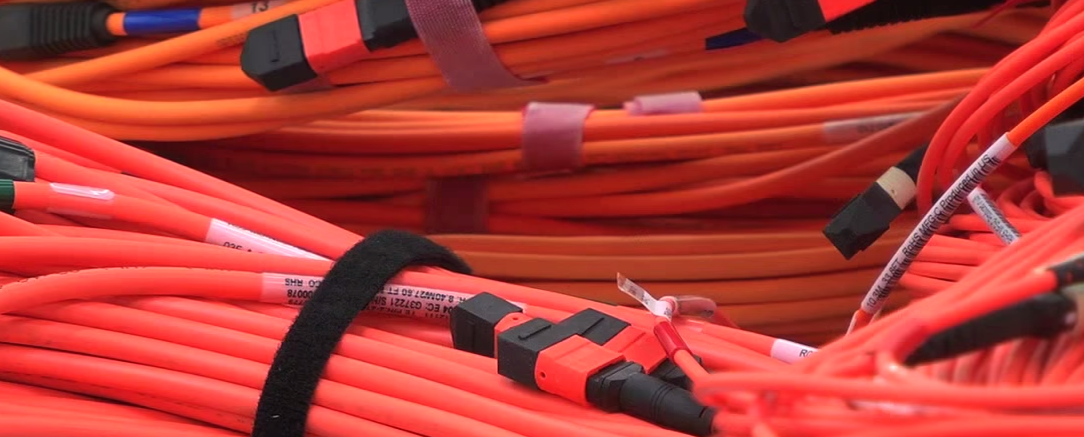
\includegraphics[width=\textwidth]{figures/bgCables.png}};
						\node (sockets) [inner sep=0, below=1.0em of cables]
						      {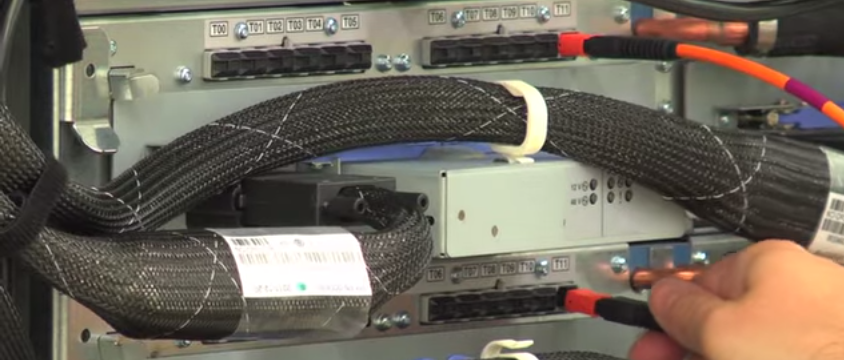
\includegraphics[width=\textwidth]{figures/bgSockets.png}};
						
						% Point at label on cable
						\draw [white, <-, line width=0.4em]
						      ([shift={(0.7cm, -0.3cm)}]cables.center)
						      -- ++(45:1cm);
						
						% Point at label on socket
						\draw [white, <-, line width=0.4em]
						      ([shift={(-1.0cm, 1.1cm)}]sockets.center)
						      -- ++(-45:1cm);
					\end{tikzpicture}
					
					\caption{Pre-labelled cables and sockets}
					\label{fig:bgWiringLabels}
				\end{subfigure}
				~
				\begin{subfigure}[t]{0.30\textwidth}
					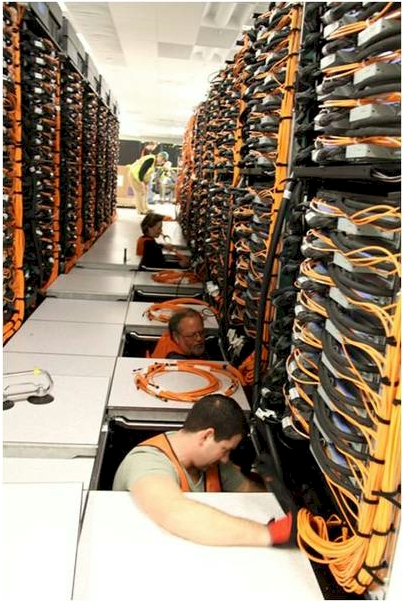
\includegraphics[height=6.15cm]{figures/bgWiring.jpg}
					
					\caption{Installation of cables}
					\label{fig:bgWiringInstallation}
				\end{subfigure}
				
				\caption[BlueGene/Q cable installation.]%
				        {BlueGene/Q cable installation~\cite{cscs13}.}
				\label{fig:bgWiring}
			\end{figure}
			
			In other large-scale architectures, the task of cable installation is
			completed by a team of technicians aided by the use of standardised
			labelling for cables and sockets as illustrated in
			figure~\ref{fig:bgWiring}~\cite{tia2006}. In these architectures the
			cabling patterns required are relatively straightforward, thanks to the
			coarseness of the units used~\cite{lakner07} or they use network
			topologies whose cabling centres around high-fan-in
			switches~\cite{cisco07,csernai15}.
			
			It has been reported in the literature that when copper cables are used,
			labour costs dominate~\cite{popa10} and while cable costs are expected to
			decline, labour costs are not~\cite{mudigonda11}. Many researchers have
			attempted to control cable installation costs by trying to reduce the
			number or length of cables required by developing alternative network
			topologies~\cite{curtis12, popa10, mudigonda11}.  Unfortunately, these
			techniques do not apply to SpiNNaker since its network topology is fixed.
			
			Supercomputer architectures such as BlueGene/Q make use of large custom
			`midplane' PCBs in place of cables to connect units within a
			cabinet~\cite{milano13}. This scheme can reduce wiring complexity since
			only coarser-grain, cabinet-to-cabinet connectivity is implemented by
			cables. Unfortunately, this technique is expensive and constrains the
			dimensions of the network topology supported by the machine. Since
			SpiNNaker is designed to scale from desktop machines to machine room
			installations, this scheme is not practical.
			
			\begin{figure}
				\center
				\begin{subfigure}[b]{0.40\textwidth}
					\begin{tikzpicture}
						\node (leds) [inner sep=0]
						      {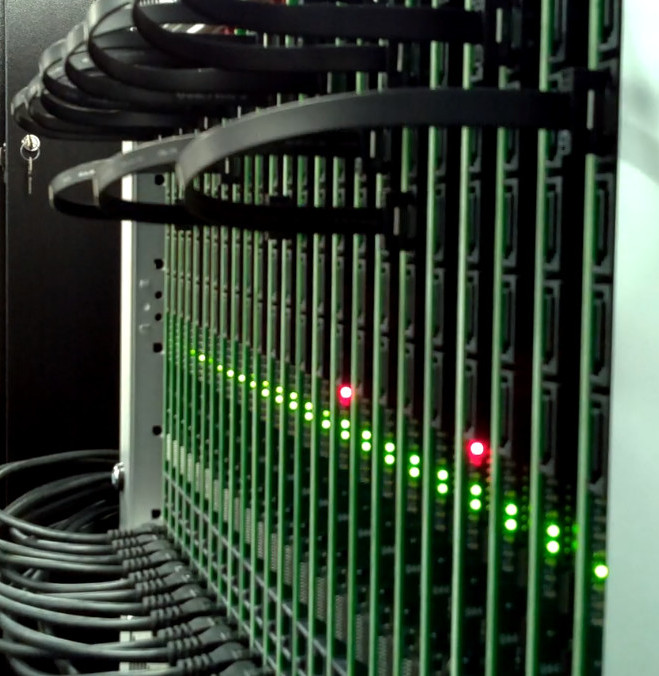
\includegraphics[width=\textwidth]{figures/leds.jpg}};
						% Point at left LED
						\draw [white, <-, line width=0.4em]
						      ([shift={(-0.0cm, -0.6cm)}]leds.center)
						      -- ++(225:1cm);
						% Point at right LED
						\draw [white, <-, line width=0.4em]
						      ([shift={(1.1cm, -1.1cm)}]leds.center)
						      -- ++(225:1cm);
					\end{tikzpicture}
					
					\caption{Diagnostic LEDs indicate the endpoints of each cable.}
					\label{fig:interactive-wiring-guide-leds}
				\end{subfigure}
				~
				\begin{subfigure}[b]{0.546\textwidth}
					\begin{tikzpicture}[thin, black!20!white]
						\node (screen) [inner sep=0]
						      {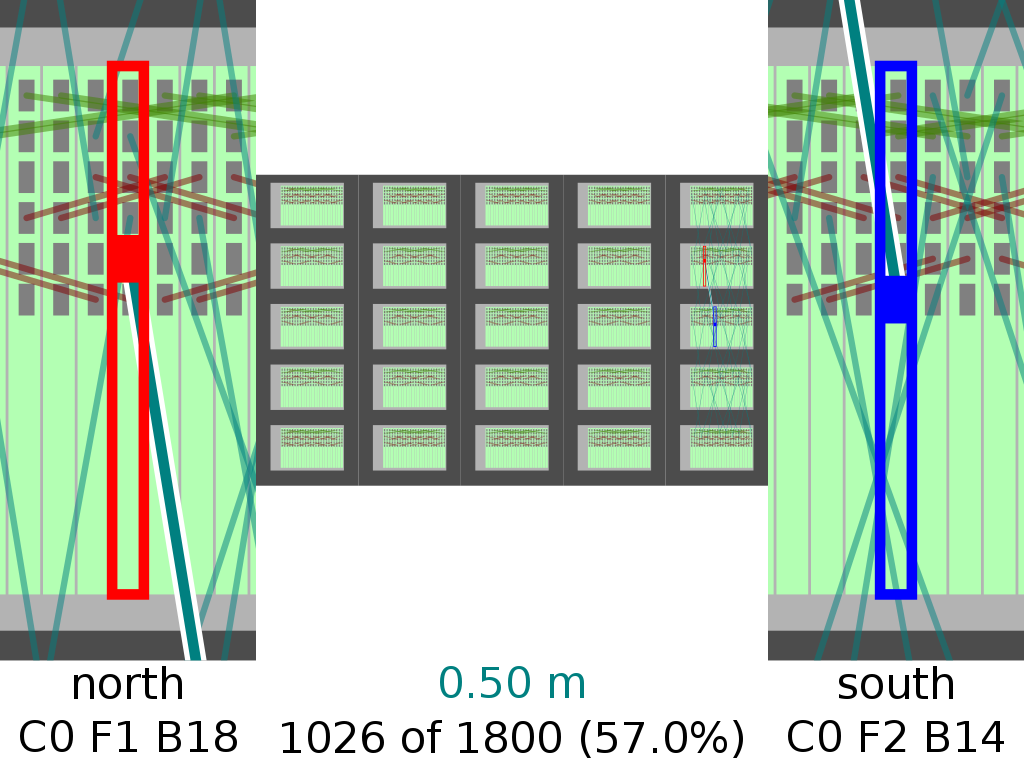
\includegraphics[width=\textwidth]{figures/wiring_guide_screenshot.png}};
						\draw (screen.south west) rectangle (screen.north east);
					\end{tikzpicture}
					
					\caption{A GUI and text-to-speech indicate what type of cable to
					install.}
					\label{fig:interactive-wiring-guide-gui}
				\end{subfigure}
				
				\caption{Interactive software guiding cable installation.}
				\label{fig:interactive-wiring-guide}
			\end{figure}
			
			Due to the high density of units in a SpiNNaker system, the detailed
			cabling patterns used can be complex, despite their overall regularity.
			To cope with this complexity, I developed a software system which employs
			diagnostic hardware built into SpiNNaker, to guide technicians through
			the cable installation process. As shown in
			figure~\ref{fig:interactive-wiring-guide}, diagnostic LEDs on each
			SpiNNaker board are used to indicate which boards to connect. The
			software also provides step-by-step cabling instructions via a Graphical
			User Interface (GUI) and audible instructions delivered via headphones.
			These instructions explicitly specify the length of cable to use for each
			connection avoiding the common problem of technicians over-estimating the
			cable length required~\cite{mazaris97}. Diagnostic registers in the
			network hardware are then used to verify the correct installation of each
			cable in real-time ensuring that mistakes are highlighted and fixed
			immediately.
			
			\begin{table}
				\center
				\begin{tabular}{lrll}
					\toprule
						Size & Cables & Time & Notes \\
					\midrule
						24 boards  & \num{72}   & \SI{10}{\minute} & \\
						1 cabinet  & \num{360}  & \SI{4}{\hour} &
							Real-time validation not used. \\
						2 cabinets & \num{720}  & \SI{2}{\hour} & \\
						5 cabinets & \num{1800} & \SI{4}{\hour} \SI{20}{\minute} &
							Three people working simultaneously. \\
					\bottomrule
				\end{tabular}
				
				\caption[Cable installation times for various SpiNNaker machines.]%
				{Cable installation times for various sizes of SpiNNaker
				machine.}
				\label{tab:install-time}
			\end{table}
			
			\begin{figure}
				\buildfig{figures/install-histogram.tex}
				
				\caption{Two cabinet SpiNNaker machine cable installation times.}
				\label{fig:install-histogram}
			\end{figure}
			
			Table~\ref{tab:install-time} shows cable installation times for various
			sizes of SpiNNaker system. The times reported do not include breaks and,
			with the exception of the five cabinet system, are for the one person
			working alone.  Figure~\ref{fig:install-histogram} shows the histogram of
			cable installation times for a two cabinet machine.  These results
			confirm the observation by Mudigonda \emph{et al.} that cables which span
			cabinets and frames take longer to install~\cite{mudigonda11}, even
			though these distances are still very short in SpiNNaker. Compared with
			commercial installation efforts, per-cable installation times are much
			shorter for SpiNNaker taking seconds compared with minutes in other
			architectures~\cite{mudigonda11}.
			
			The positive impact of real-time validation of installed cables can
			clearly be seen by comparing the installation times of the one and two
			cabinet systems. Though double the size, the two cabinet machine was
			built in half the time required to build the single cabinet machine.
			While building the smaller machine, real-time cable validation had not
			yet been implemented and the installation process was interrupted for
			several minutes every time a misplaced connection was discovered.
			
			In the three-person cable installation effort employed for the five
			cabinet system, the guidance software was configured to assign each
			technician cables in non-overlapping parts of the machine ensuring
			minimal interference between the technicians. As expected, this renders
			the problem embarrassingly parallel, as in commercial computer
			installations.
			
			\begin{figure}
				\center
				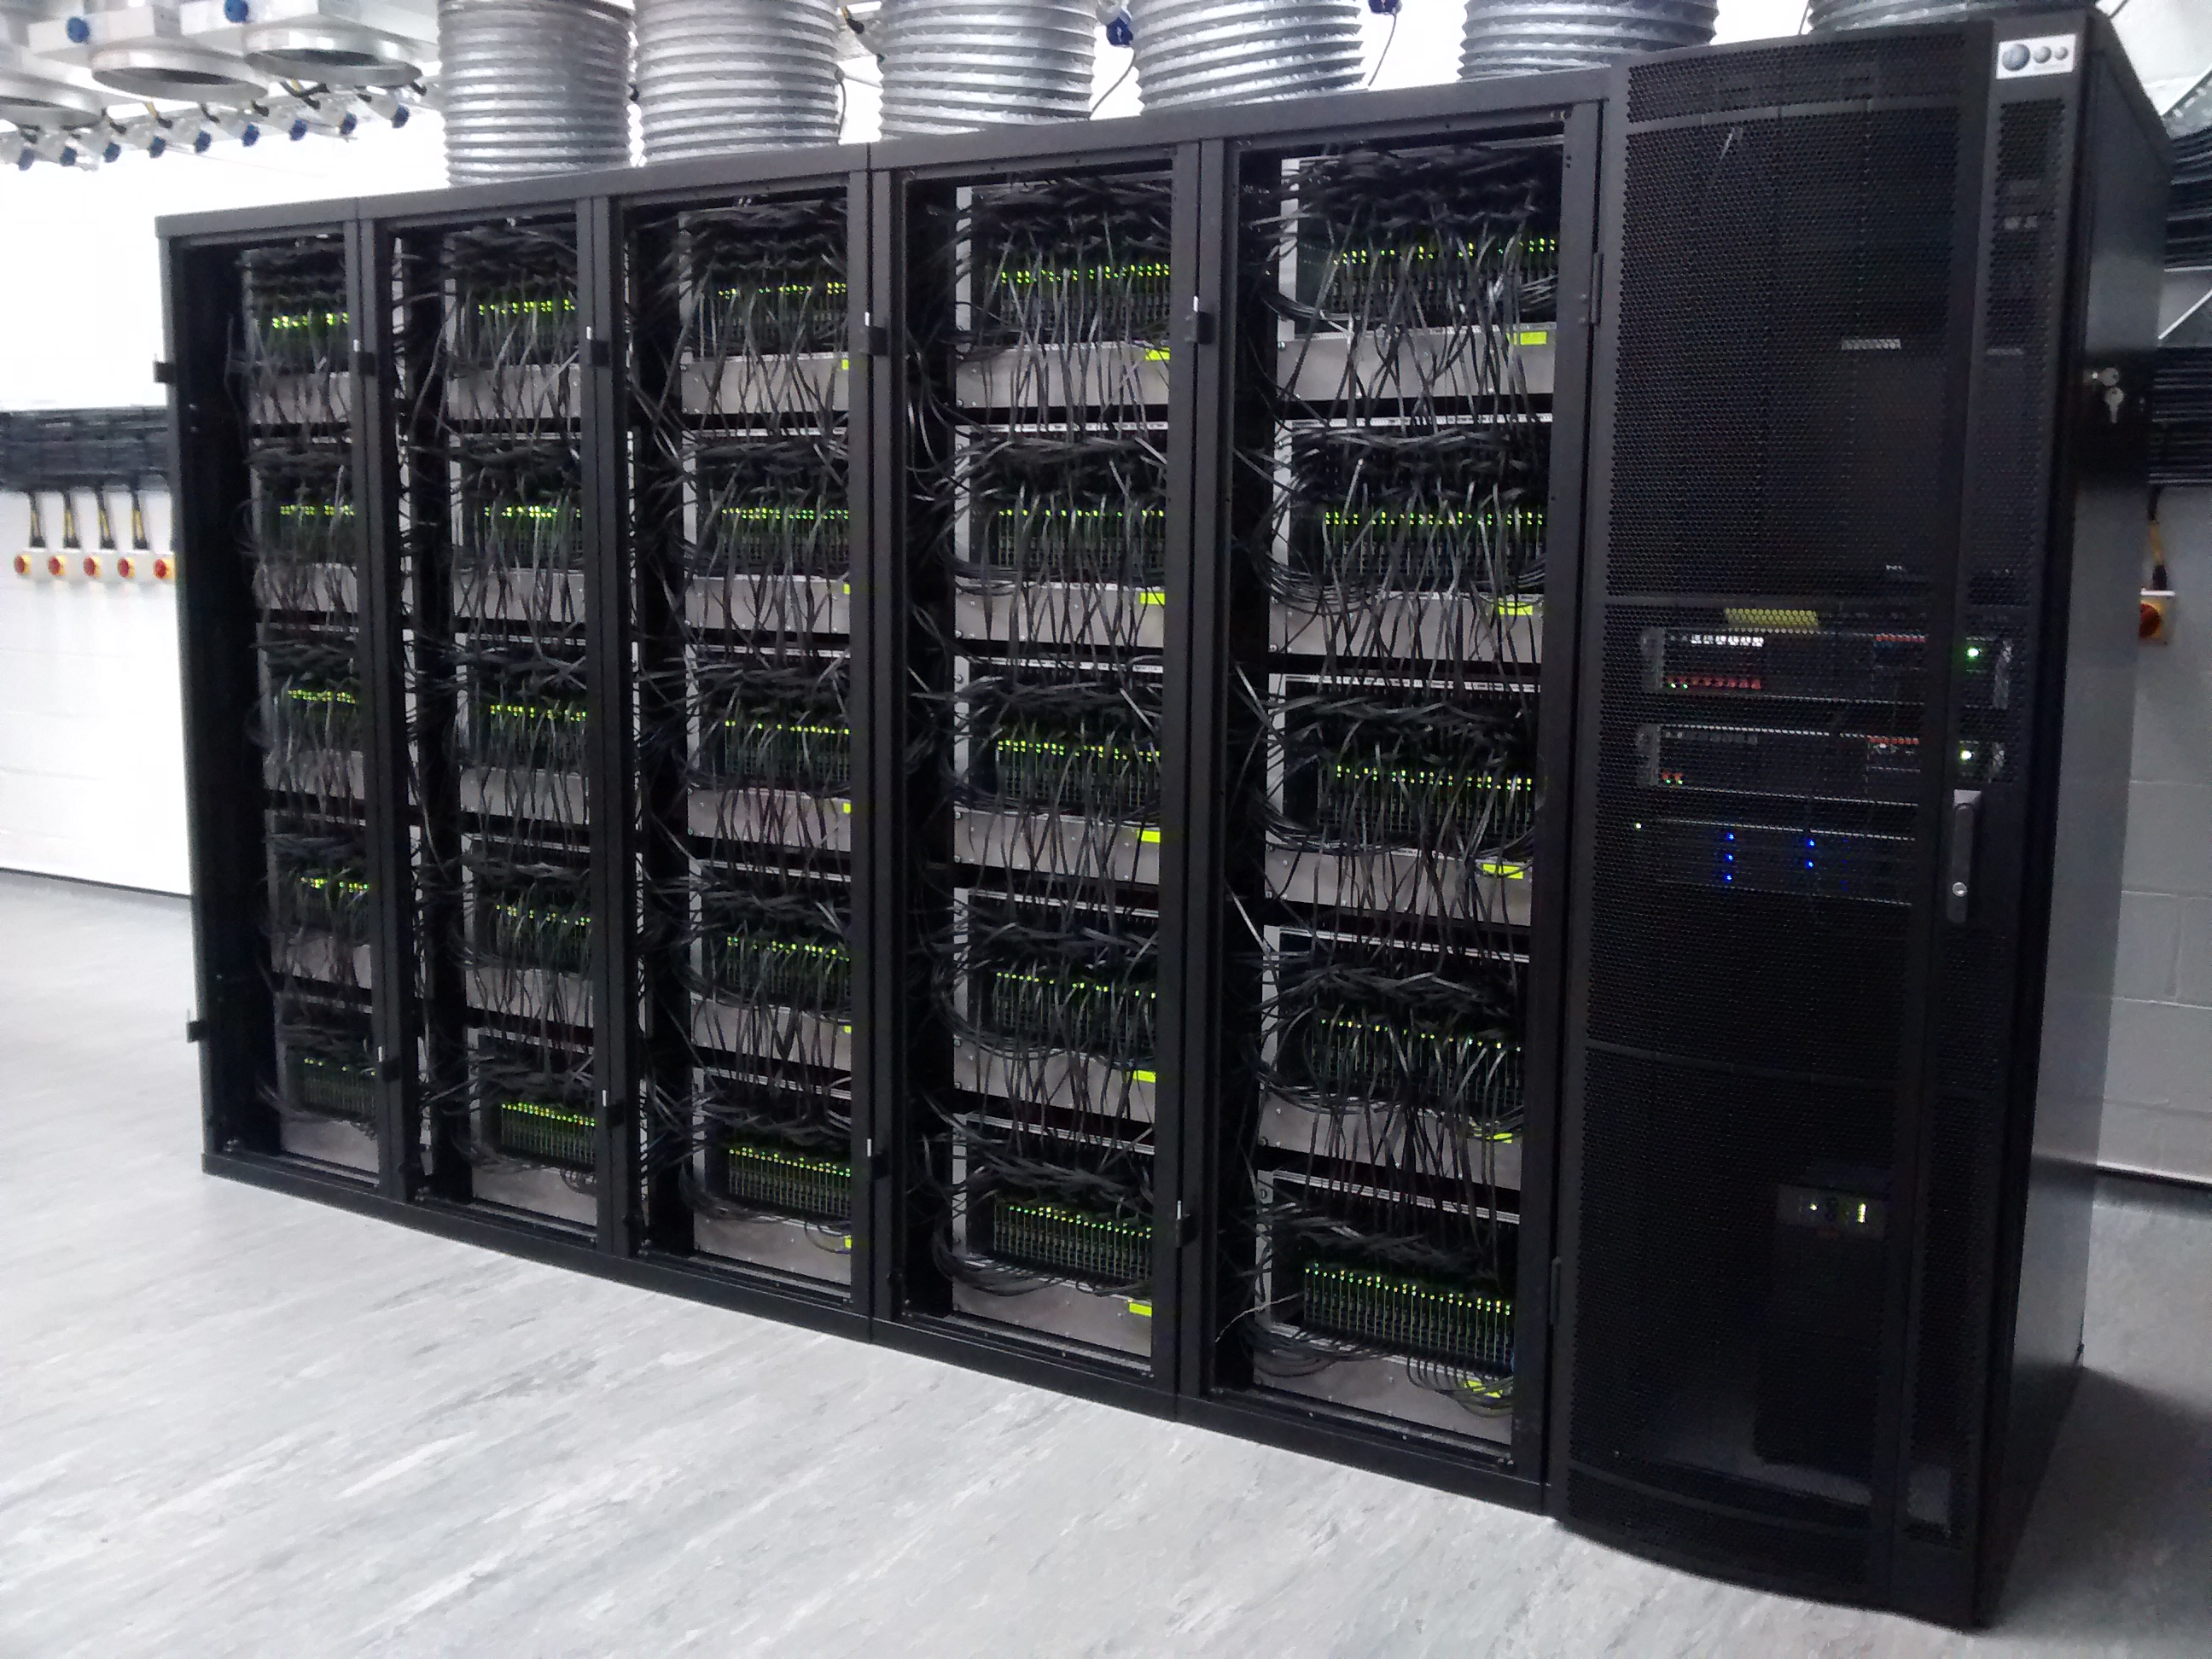
\includegraphics[width=0.8\linewidth]{figures/halfMillionCoreComplete.jpg}
				
				\caption[The five cabinet SpiNNaker system.]%
				{The five cabinet SpiNNaker system. The cabinet on the right contains
				conventional host servers which control SpiNNaker.}
				\label{fig:halfMillionCoreComplete}
			\end{figure}
			
			The completed five cabinet system is photographed in
			figure~\ref{fig:halfMillionCoreComplete}. A time-lapse video showing the
			construction and cable installation of this machine is also available on
			YouTube~\cite{heathcote16}.
			
		\subsection{Thermal implications}
			
			In large SpiNNaker machines, each 24 board frame contains a fan tray
			which pulls cool air from the front of the frame, between the SpiNNaker
			boards. The warmed air is then ejected out of the rear of the frame where
			ducting directs it into industrial chillers. Conventional guidance on
			data centre design suggests that routing cables in the path of the
			system's airflow can have a serious impact on cooling
			performance~\cite{cisco07}.  To determine what effect the cabling
			described in this chapter had on SpiNNaker's cooling, a test program was
			executed to simulate heavy load before and after cable installation. The
			temperatures reported by the sensors on the top of each SpiNNaker board
			were sampled at regular intervals and once the overall system temperature
			stabilised, the mean temperature was recorded.
			
			Before the cabling was installed, the temperature stabilised at
			\SI{49}{\celsius} while after installation it stabilised at
			\SI{42}{\celsius}.
			
			These two data points suggest that the system's temperature is unlikely
			to have been been seriously impacted by cable installation. Since the two
			experiments were run on different days (with potentially different
			ambient temperatures) and are based on a single experiment, it is not
			possible to infer much more from this result.
			
		\subsection{Maintenance}
			
			At the time of writing, the five cabinet machine is still being
			commissioned and so the long term maintenance impact of the system's
			cabling is not known. One important factor in the maintainability of the
			system is the ease with which faulty boards can be replaced. During
			commissioning a number of boards have been replaced by someone not
			involved in the machine's installation. Informal measurements suggest
			that boards near the centre of a frame (i.e. those most likely to be
			blocked by unrelated cables) take around ten minutes to replace,
			including time spent removing and replacing cables obstructing the board
			being exchanged. By comparison boards at the edge of the machine take
			around six minutes to replace. Though similar timing reports are
			unavailable for other architectures, these times appear reasonable in
			practice and suggest maintenance is not impaired by the wiring plan used.
		
		\subsection{Verification}
			
			The real-time cabling verification process ensures that each board is
			connected correctly to its neighbours according to the cabling pattern
			described in this chapter. To verify that this pattern actually
			implements the desired hexagonal torus topology, SpiNNaker's system
			software was upgraded to check the correctness of the network topology
			during boot.
			
			When the system is first booted a single chip is assigned the coordinate
			$(0, 0, 0)$. From this, its six neighbouring chips may in turn discover
			their own locations in the topology, followed by their neighbours and so
			on. Eventually every chip knows its location. If the cabling scheme does
			not form a valid hexagonal torus topology, some chips will be assigned
			conflicting coordinates, causing a boot error.
			
			All of the SpiNNaker machines constructed were found to have the correct
			network topology. Furthermore, the machines constructed have been used
			successfully in practice, including in later work described in
			chapters~\ref{sec:routing} and~\ref{sec:placement}.
	
	\section{Conclusions}
		
		In this chapter I presented a practical method of constructing real-world
		installations of large hexagonal torus topologies such that long cables
		spanning the width and height of the system are not required. Two
		transformations, shearing and slicing, are presented which allow
		conventional network folding techniques to be applied to hexagonal toruses
		to eliminate long `wrap-around' links. Though both techniques incur some
		overhead in terms of mean and maximum cable length, the maximum cable
		length does not grow with the size of the network. This result makes
		hexagonal torus topologies a practical and scalable choice for future
		systems.
		
		The theoretical results presented in this chapter have been confirmed
		through the successful construction of several large-scale SpiNNaker
		machines which implement hexagonal torus topologies. During construction,
		diagnostic features of SpiNNaker's hardware were employed to guide
		technicians performing cable installation. This technique was found to be
		highly effective with cable installation times measured in seconds rather
		than minutes as reported for other architectures. Surprisingly there was no
		evidence found of this technique being applied to other architectures and
		consequently this secondary result may be of interest for future research.
